\documentclass[a4paper]{article}

%\newcommand{\addbibresource}[1]{}
%\newcommand{\printbibliography}{}
\usepackage[style=ieee,sorting=none,dateabbrev=false,backend=biber]{biblatex}
\usepackage[english]{babel}
\usepackage[utf8]{inputenc}
\usepackage{amsmath}
\usepackage{graphicx}
\usepackage{parskip}
\usepackage{amssymb}
\usepackage{upgreek}
\usepackage{todonotes}
\usepackage{csquotes}
\usepackage{pdfpages}

\addbibresource{report.bib}

\setcounter{secnumdepth}{5}
\newcommand{\subsubsubsection}[1]{\paragraph{#1} \mbox{}}
\newcommand{\subsubsubsubsection}[1]{\subparagraph{#1} \mbox{}}

\newcommand\Forall{\mathop{\mbox{\Large $\mathsurround0pt\forall$}}}


\title{Complex Task Allocation: A Comparison of Metaheuristics}
\author{
	Group 27 \\
	\\
	Lucas Wojciechowksi, Ariel Weingarten, Alexander Maguire, \\
	Austin Dobrik, Dane Carr}
\date{\today}

\begin{document}

\maketitle

\listoftodos

\section*{Summary}

This report is an analysis of the efficacy of different metaheuristic algorithms in solving a complex task allocation problem.
Complex task allocation is the assignment of complex and simple tasks to a group of robots. This report is taking an optimization-based approach to solve a multi-task robot, single-robot task, instantaneous assignment version of the multirobot task assignment problem that adopts a decompose-then-allocate strategy to handle complex tasks.

Five metaheuristic algorithms were tested for this report. They are: Tabu Search, Simulated Annealing, Genetic Algorithms, Particle Swarm Optimization, and Ant Colony Optimization.

Unfortunately, we were unable to find a canonical dataset for this problem, and thus have run these algorithms on a randomly-generated dataset. An example of the reduced dataset used is included in Section 3.3, with the larger datasets on the attached digital media.

The results of experimentation are as follows. The algorithm that produced the best solution was Simulated Annealing, at the cost of a relatively large number of iterations to achieve convergence.

If computation time needs to be minimized, then Tabu Search is able to produce the best solution in the shortest amount of time -- though its solutions are inferior to those produced by Simulated Annealing.

In conclusions, this report recommends the use of Simulated Annealing for the purposes of Complex Task Allocation.

\section{Introduction}

\subsection{Problem Context}

As the digital revolution accelerates, electronics have become more than passive desktop appliances --- robotics has given computers a means to interact with the world around them, greatly expanding the scope of the tasks we can make them perform.

Robots, like people, are more effective at many types of tasks when cooperating in a group rather than working alone. For this reason, multirobot systems (MRS) are becoming a high interest subject. An MRS is a group of robots that are designed to perform a collective behavior.

We define a ``heterogeneous MRS" to be a group of different types of robots, some more adept at certain tasks than others. In this paper, we will refer to a heterogeneous MRS simply as an MRS.

There are numerous advantages of using an MRS over using a single multi-purpose robot. For example, it is simpler to design a robust single purpose robot than a robot with multiple abilities and configurations. Simple designs tend to be more robust and lead to more reliable robots. Another source of reliability is that an MRS can have redundancies; if one robot fails, another may resume its tasks.  In addition, many complex tasks are distributed over a large area and would be slow to accomplish with a single robot.

Tasks particularly well suited to MRSs include
\begin{itemize}
\item search and rescue in dangerous environments
\item surveillance
\item space construction
\end{itemize}


\subsection{Problem}

In this report, we will determine the strengths and weaknesses of different metaheuristic algorithms in finding near-optimal solutions to complex task allocation problems. Complex task allocation, as defined in this assignment's problem statement, is:
\begin{quote}
  In mobile surveillance systems, complex task allocation addresses how to optimally assign a set of surveillance tasks to a set of mobile sensing agents to maximize overall expected performance, taking into account the priorities of the tasks and the skill ratings of the mobile robots.
\end{quote}

Replacing humans with robots in surveillance tasks -- and allocating those robots efficiently -- is important because areas under surveillance usually possess a high degree of danger.

Efficiently finding near-optimal solutions to complex task allocation has broad implications beyond surveillance. In essence, this report answers the question ``which robot should perform which task?''\cite{Badreldin}


\subsection{Report Structure and Direction}

This report is being written as an assignment for the University of Waterloo's ECE457a course, ``cooperative and adaptive algorithms."

In this paper, we determine the strengths and weaknesses of different metaheuristic algorithms in finding near-optimal solutions to Complex Task Allocation problems. The metaheuristic algorithms under consideration are:
\begin{itemize}
\item tabu search (TS)
\item simulated annealing (SA)
\item genetic algorithms (GA)
\item particle swarm optimization (PSO)
\item ant colony optimization (ACO)
\end{itemize}

We will begin with a review of existing literature on the subject. Next, this report will present a problem formulation and model from which we will implement our algorithms.

The paper then describes how the well-known Traveling Salesman Problem can be adjusted for use with Complex Task Allocation, and from there, identifies the criteria upon which each metaheuristic technique's performance is to be evaluated.

Afterwards, the results of running each technique are then presented against these performance criteria, and finally conclusions are drawn, with recommendations for future work.

\newpage
\section{Literature Review}

An examination of existing literature reveals two predominant schools of approach to solving Multi-Robot Task Allocation (MRTA). There are market-based and optimization-based approaches.

The market-based approach is inspired from the development of market economies in human societies.
Each robot is made analogous to an individual seeking profit within a market and as a result, effecting a redistribution of resources within the environment.

The optimization-based approach is rooted in mathematics rather than socio-economic observation.
The thrust of which is to identify an equation that captures the constraints contained in a problem and to find a solution that either maximizes the profit or minimizes the cost of a given solution.

The goal of this report is to perform a comparative study of metaheuristic techniques and so this directs the attention of the paper towards an optimization-based approach for solving MRTA. However, this is not the only approach; Khamis et al.\cite{Khamis} propose a method for using a market-based approach to generate candidate solutions that are then fed into a metaheuristic algorithm, but it will not be used here.\\

In ``Complex Task Allocation in Mobile Surveillance Systems''\cite{Khamis}, Khamis et al. describe a taxonomy for classifying MRTA problems examined in literature. From their taxonomy, the MRTA problem examined by this report has the following classifications:

\begin{enumerate}
\item Multi-task robots: Each robot is able to perform various tasks, and has a certain skill at each type of task.
\item Single-robot tasks: Each task can be completed by a single robot.
\item Instantaneous Assignment: The assignment of tasks to robots will be calculated once and will not be updated dynamically as the robots execute their given task list.
\end{enumerate}

The scope of this report will focus on a decompose-then-allocate approach towards complex tasks. That is, all complex tasks will be broken up into subtasks that will then be assigned out to particular robots. This makes a strong assumption about the independence of the subtasks, but is not without precedence in the literature.\cite{Khamis}\\

In Gerkey's ``A Framework for Studying Multirobot Task Allocation''\cite{Gerkey}, he identifies MRTA as an instance of the Optimal Assignment Problem (OAP). The OAP considers $n$ workers who have various skill levels at $m$ jobs that must be completed, and seeks a mapping of workers to jobs that optimizes overall performance. At first this seems like an ideal problem onto which to map MRTA, but there are a few shortcomings for the particular instance of MRTA being studied in this report: robots are not being assigned to a single task, but rather are given a tour of several tasks through a given area of interest.

The importance of considering distance traveled, in addition to the cost associated in a task-robot assignment make the mapping onto Traveling Salesman Problem (TSP) a more natural fit.\\

This report makes use of the multiple Travelling Salesman Problem (mTSP) formulation as described by Badreldin, Hussein, and Khamis with some important differences:\cite{Badreldin}

Instead of including a robot aging factor, an energy capacity feature has been identified to put a harder constraint on robot tour lengths. In addition, instead of considering a minimum task completion time that holds for all robots, each type of robot has its own task completion time. This explicitly decouples a robot's skill at a task from the time it takes to complete the task. It also more accurately represents that different types of robots can have radically different methods for accomplishing the same task. To reconcile this change with the idea that tasks have certain requirements, a time of infinity is assigned to robots who lack any skill at a particular task.

\newpage
\section{Problem Formulation and Modeling}

\subsection{Problem Formulation}

Suppose we have a set of tasks, $\{1, 2, ..., n_\mathit{tasks}\}$, which need to be completed by a set of robots, $\{1, 2, ..., n_\mathit{robots}\}$.

We seek a solution $S$ that consists of assigning each robot an ordered set of tasks to complete (known as a ``tour"), such that each task is performed by exactly one robot. Additionally, we aim to minimize the overall cost of the solution. Each tour begins and ends at the robot's ``home".

The notion of a $robot$'s path is formalized as:
$$
\Forall_{r=0}^{n_\mathit{robots}}
S(r) = \{ \mathit{home}(r), t_1, t_2, ..., t_n, \mathit{home}(r) \}
$$

\subsubsection{Canonical Solution Representations}
The overall solution $S$ has a canonical vector representation as an n-tuple, consisting of a permutation of the set:
$$
\{1, 2, \dots n_{tasks}\} \cup \{0\}^{n_{robots}-1}
$$

This tuple is read from left to right, and describes the concatenation of each $robot_i$'s path, using 0 to mark the end of a path. This 0 is henceforth known as a sentinel value. This representation \textbf{does not} include $robot_i$ starting at or returning to $\mathit{home}(i)$, since this information is redundant by the problem definition.

To help cement this important representation in the reader's mind, consider the following canonical solution vector:
$$
\{3,4,2,0,0,1,5\}
$$
which should be interpreted as
\begin{itemize}
\item $S(1) = \{ \mathit{home}(1), 3, 4, 2, \mathit{home}(1) \}$
\item $S(2) = \{ \mathit{home}(2), \mathit{home}(2) \}$
\item $S(3) = \{ \mathit{home}(3), 1, 5, \mathit{home}(3) \}$
\end{itemize}

\subsubsection{Data Homogeneity}

For simplicity and homogeneity of internal data models, we represent homes as tasks:
$$\mathit{home}(r) = n_\mathit{tasks} + r$$

subject to the following constraints:
$$
\mathit{task\,time}(\mathit{home}(i)) = 0 \qquad \forall i \in \mathit{robots}
$$
$$
\mathit{priority}(\mathit{home}(i)) = 0 \qquad \forall i \in \mathit{robots}
$$
$$
\mathit{distance}(\mathit{home}(i), \mathit{home}(j)) = 0 \qquad \forall i, j \in \mathit{robots}
$$


\subsubsection{Overall Cost}

We will consider a multi-objective cost function, $\mathit{cost}$, that accounts for
\begin{enumerate}
\item $\mathit{cost}_\mathit{time}$, how long it takes to complete all tasks, assuming the robots work in parallel
\item $\mathit{cost}_\mathit{energy}$, whether or not each robot is able to complete its tour before running out of ``energy"
\item $\mathit{cost}_\mathit{quality}$, how well the tasks are completed relative to their priorities
\end{enumerate}

We define overall $\mathit{cost}$ as a linear combination of these cost functions, introducing two constants, $\alpha$ and $\beta$.
$$
\mathit{cost}(S) =
  \alpha \beta \, \mathit{cost}_\mathit{time}(S) +
  (1-\alpha) \mathit{cost}_\mathit{quality}(S) +
  \mathit{cost}_\mathit{energy}(S)
$$

$\alpha$ is a tuning parameter allowing for the relative importance of quality vs time to be adjusted. $\alpha = 1$ places all emphasis on time; $\alpha = 0$ places all emphasis on quality.

$\beta$ is a normalization parameter that makes $\mathit{cost}_\mathit{time}$ directly comparable to $\mathit{cost}_\mathit{quality}$. It is discussed in more detail in the next section.

\subsubsection{Time Cost}

The time it takes to travel between tasks is a function of ``distance" and ``velocity." Each robot, $r$, may travel at a different velocity, measured in units distance per units time.
$$\mathit{velocity}(r) > 0, \in \mathbb{R}$$
Each task, $t$, may be a different distance from each other task, $u$. For simplicity, we represent home locations as tasks.
$$\mathit{distance}(t, u) \ge 0, \in \mathbb{R}$$

Additionally, each robot $r$ may complete each task $t$, in a different amount of time.
$$\mathit{task \, time}(r, t) > 0, \in \mathbb{R}$$

The total amount of time it takes for a robot $r$, to complete a tour $P$, is given by:
$$
\mathit{tour \, time}(r, P) =
  \left(
    \sum^{|P|}_{t=2} \mathit{distance}(t - 1, t) \cdot \mathit{velocity}(r)
  \right) +
  \left(
    \sum^{|P|}_{t=1} \mathit{task \, time}(r, t)
  \right)
$$

We define $\mathit{cost}_\mathit{time}$ as the amount of time it takes to complete all tasks, assuming the robots work in parallel; effectively the max tour time across all robots.
$$
\mathit{cost}_\mathit{time}(S) =
  \max_{r=1}^{n_\mathit{robots}}
  \mathit{tour \, time}(r, S(r))
$$

In the overall cost function, $\beta$ is a normalization parameter that makes $\mathit{cost}_\mathit{time}$ directly comparable to $\mathit{cost}_\mathit{quality}$. Because skills and priorities are bounded $\in [0, 1]$, we are guaranteed that, for some tour $P$ and some robot $r$, $\mathit{cost}_\mathit{quality}(r, P) \in [0, |P|]$. To make $\mathit{cost}_\mathit{time}$ directly comparable to $\mathit{cost}_\mathit{quality}$, we must scale $\mathit{cost}_\mathit{time}$ using $\beta$ such that it has the same bounds, $\in [0, |P|]$. Such a $\beta$ may be calculated as
$$
\beta =
    \frac
      {n_\textit{robots}}
      {
        2 \cdot
        \max \left(
          \frac
            { \max\limits_{r=1}^{n_\mathit{robots}} \max\limits_{t=1}^{n_\mathit{tasks}} \mathit{distance}(r, t) }
            { \min\limits_{r=1}^{n_\mathit{robots}} \mathit{velocity}(r) },
          \max\limits_{r=1}^{n_\mathit{robots}} \max\limits_{t=1}^{n_\mathit{tasks}} \mathit{task \, time}(r, t)
        \right)
      }
$$

\subsubsection{Energy Cost}

Each robot, $r$, may be capable of spending a different amount of time on tour. One unit energy equates to the ability to spend one additional unit time on tour.
$$\mathit{energy}(r) > 0, \in \mathbb{R}$$

We define $\mathit{cost}_\mathit{energy}$ to evaluate to 0 if this hard constraint is met for all robots, and $\infty$ otherwise
$$
\mathit{cost}_\mathit{energy}(S) = \begin{cases}
0 & \text{if } \mathop{\forall}\limits_{r=0}^{n_\mathit{robots}} \mathit{energy}(r) \geq \mathit{tour \, time}(r, S(r)) \\
\infty & \text{otherwise}
\end{cases}
$$

\subsubsection{Quality Cost}

We define $\mathit{cost}_\mathit{quality}$ to represent the skill with which each task was done relative to that task's priority. This is quantified as the sum of all the products of the skill with which a task was done by the priority that task had.
$$
\mathit{cost}_\mathit{quality}(S) =
  \sum^{n_\mathit{robots}}_{r=1}
  \sum^{|S(r)|}_{t=1}
  1 - \mathit{priority}(r, t) \cdot \mathit{skill}(r, t)
$$
Since performing a high priority task with a highly skilled robot is desirable and we want to minimize cost, we subtract the maximum possible value, 1, from the product of the priority and skill (recall that $\mathit{skill}(r) \in [0, 1]$ and $\mathit{priority}(r, t) \in [0, 1]$).


\subsection{Modeling as Traveling Salesman Problem (TSP)}

\subsubsection{Adaptation}
The area of interest for the robots in the MRS can be represented as a two dimensional bounded space. Within this space, the location of tasks and robot home locations can be represented as a graph. As described in the previous section, the goal is to create an assignment of tasks to robots which minimizes the total cost of travel. This makes the MRTA problem a good fit for reduction to the mTSP problem. This report will be making use of some well-studied variations of mTSP.\cite{Badreldin}
\begin{enumerate}
\item \textbf{Salesmen starting node}: Robots are not guaranteed to start from the same node and must end their tour by returning to their starting node.
\item \textbf{Number of salesmen}: The number of robots can vary between instances of this problem, but is static for the duration of any given instance.
\item \textbf{City time frame}: Robots take a certain amount of time to complete a task and therefore spend a certain amount of time at a given node.
\item \textbf{Fair division of salesmen}: There are constraints on the maximum amount of work that a robot can perform on their tour and so the required traveling should be distributed amongst the available agents in a relatively fair manner as defined by the problem parameters.
\end{enumerate}

In an MRS, there is heterogeneity in robot composition. This requires the augmentation of the ``salesman'' idea to support some differentiating factors. This report has identified 4 main features:

\begin{enumerate}
\item \textbf{Velocity}: Each robot has a speed at which they travel between tasks.
\item \textbf{Energy}: Each robot has an energy capacity that restricts how long it can be away from its home node.
\item \textbf{Skill}: Each robot has a skill rating that represents its ability to complete a task.
\item \textbf{Task Completion Time}: Robots do not necessarily take the same amount of time to complete a task.

\end{enumerate}

In this MRTA problem, there is also heterogeneity in the tasks that are assigned to visit. For this reason, the idea of ``cities'' have been augmented with the following features\todo{there's only one feature}:

\begin{enumerate}
\item \textbf{Priority}: Some tasks are more important that others and should be considered first.
\end{enumerate}

The next section describes the graph that will be constructed for use with mTSP.

\subsubsection{The Graph}
We will model complex task allocation loosely on the traveling salesman problem.

Given a population of $\mathit{robots}$, a set of $\mathit{tasks}$, a set of $\mathit{homes}$, a priority for each task $P$, each robot's skill at performing each task $M_{skill}(r,t)$ and an ordered assignment of tasks to robots $S(r)$, for each $r \in \mathit{robots}$
we can create a directed, weighted graph as follows:

Given a random initial solution, $S_0$,

\begin{align*}
	G &= (V, E) \\
	V &= \mathit{homes} \cup \mathit{tasks} \\
	E_{i, j} &= distance(i,j) \qquad \forall i,j \in [1, n_{robots}+n_{tasks}] \\
\end{align*}
%

That is, we create a graph that shows the distances between every task and the distances between every task and every home.

From here, we can run TSP on the created graph. The cost of taking each edge will be determined using $w$ which will take in the distance represented by that edge as an input. Every robot starts at their home.

\subsection{Reduced Size Problem}

In this section, we define a reduced size complex task allocation problem which
will be used to perform hand-iterations of various optimization algorithms in
the following sections.

Suppose we have two robots with the following attributes:

\begin{center}
\begin{tabular}{lll}
        & \textbf{velocity} & \textbf{energy} \\
\textbf{robot 1} & 0.9146   & 58.2024          \\
\textbf{robot 2} & 0.6509   & 45.0418
\end{tabular}
\end{center}
\vspace{1em}

These robots must complete three tasks:

\begin{center}
\begin{tabular}{llllll}
                &                   & \textbf{robot 1} & \textbf{robot 1} & \textbf{robot 2} & \textbf{robot 2} \\
                & \textbf{priority} & \textbf{skill}   & \textbf{time}    & \textbf{skill}   & \textbf{time} \\
\textbf{task 1} & 0.7761            & 0.97195          & 2.5511           & 0.33896          & 6.1632        \\
\textbf{task 2} & 0.3663            & 0.46364          & 8.8416           & 0.44659          & 3.7353        \\
\textbf{task 3} & 0.8863            & 0.83202          & 6.1189           & 0.02791          & 3.0623
\end{tabular}
\end{center}
\vspace{1em}

The distances between tasks and home locations are:

\begin{center}
\begin{tabular}{llllll}
                & \textbf{task 1} & \textbf{task 2} & \textbf{task 3} & \textbf{home 1} & \textbf{home 2} \\
\textbf{task 1} &   -             & 3.7604          & 6.2783          & 9.3271          & 1.4957 \\
\textbf{task 2} & 8.0510          &   -             & 8.4473          & 1.3190          & 4.9917 \\
\textbf{task 3} & 3.2972          & 8.5977          &   -             & 8.5270          & 0.4359 \\
\textbf{home 1} & 2.5143          & 8.4739          & 4.6241          &    -            &    -   \\
\textbf{home 2} & 1.2170          & 6.1530          & 3.9628          &    -            &    -
\end{tabular}
\end{center}

\newpage
\section{Proposed Solution}

In this section, we will consider five metahuristics in the context of complex task allocation:
\begin{itemize}
\item tabu search
\item simulated annealing
\item genetic algorithm
\item particle swarm optimization
\item ant colony optimization
\end{itemize}

In the following subsections, we will, for each metaheuristic, provide a brief
high level description of the algorithm, show and explain two ``hand iterations"
on the reduced problem, and provide a Matlab implementation.

All hand iterations will use $\alpha = 0.5$, treating time and quality costs
equally, and $\beta = 0.06979$, calculated as specified in section 3.2.1. Where applicable
we will use the ``randomly" selected initial solution, $S_0 = [ 1, 2, 0, 3 ]$.

\subsection{Tabu Search Algorithm} % Lucas

Tabu Search was the first proposed metaheuristic\cite{GloverTabu} and, as such, is a very simple algorithm --- it takes a similar approach to  hill climbing in that it starts with a random solution and seeks the optimal solution by continually moving towards improving neighbor solutions. It improves on hill climbing, however, with the addition of a tabu list. The tabu list ``remembers" recent moves and discourages backtracking, helping the algorithm to avoid becoming stuck in a local optima.

One technique for using tabu search to solve permutation problems -- like this formulation of complex task allocation -- is described by Glover and Laguna in ``Modern Heuristic Techniques for Combinatorial Problems"\cite{GloverModern}.

We begin with a random solution, represented as a canonical solution vector. Next, we find a number of random neighboring solutions, where a neighboring solution is defined as one that can be obtained by swapping two elements. The neighbor with the lowest cost is then chosen, preferring non-tabued solutions over tabued ones, and update the tabu list to mark the swapped positions for some number of future iterations. This process is repeated until some stopping criteria is met.

\subsubsection{Hand Iterations}

In these hand iterations, we will use a tabu tenure of 1 and and aspiration criteria that allows globally improving but tabu solutions to be considered, without updating their tenure.

\subsubsubsection{Iteration 1}

We begin with our randomly selected initial solution, and initial global best
$$S_\textit{best} = S_0 = [ 1, 2, 0, 3 ], \; \textit{cost}(S_\textit{best}) = 3.1617$$

Next, we find all neighboring solutions and evaluate the cost of each. No solutions are tabu yet because our tabu list is empty
\begin{center}
\begin{tabular}{lllll}
& \textbf{swap}   & \textbf{solution}    & \textbf{tabu?} & \textbf{cost}  \\
$S_{1,1}$ & $1,2$ & $[2, 1, 0, 3]$ & no & $3.8583$ \\
$S_{1,2}$ & $1,3$ & $[0, 2, 1, 3]$ & no & $\infty$ \\
$S_{1,3}$ & $1,4$ & $[3, 2, 0, 1]$ & no & $3.6619$ \\
$S_{1,4}$ & $2,3$ & $[1, 0, 2, 3]$ & no & $3.5146$ \\
$S_{1,5}$ & $2,4$ & $[1, 3, 0, 2]$ & no & $3.7910$ \\
$S_{1,6}$ & $3,4$ & $[1, 2, 3, 0]$ & no & $4.3288$ \\
\end{tabular}
\end{center}
\vspace{1.5em}

Observe that $S_{1,4}$ has the lowest cost and is not tabu. Therefore, we let
$$S_{1, \textit{best}} = S_{1,4} = [1, 0, 2, 3], \; \textit{cost}(S_{1, \textit{best}}) = 3.6619$$
However, $S_\textit{best}$ is not updated because $S_{1, \textit{best}}$'s cost is higher.

Since this solution was created by swapping elements 2 and 3 in $S_0$, we mark those in our tabu list with a tenure of 1
\begin{center}
\begin{tabular}{lllll}
\textbf{position} & 1 & 2 & 3 & 4 \\
\textbf{tenure}   & 0 & 1 & 1 & 0
\end{tabular}
\end{center}
\vspace{1.5em}

\subsubsubsection{Iteration 2}

We begin by finding all neighboring solutions of $S_{1, \text{best}} = [1, 0, 2, 3]$
\begin{center}
\begin{tabular}{lllll}
& \textbf{swap}   & \textbf{solution}    & \textbf{tabu?} & \textbf{cost}  \\
$S_{2,1}$ & $1,2$ & $[0, 1, 2, 3]$ & yes & 3.4210 \\
$S_{2,2}$ & $1,3$ & $[2, 0, 1, 3]$ & yes & 2.9759 \\
$S_{2,3}$ & $1,4$ & $[3, 0, 2, 1]$ & no  & 3.7690 \\
$S_{2,4}$ & $2,3$ & $[1, 2, 0, 3]$ & yes & 3.1617 \\
$S_{2,5}$ & $2,4$ & $[1, 3, 2, 0]$ & yes & 4.1556 \\
$S_{2,6}$ & $3,4$ & $[1, 0, 3, 2]$ & yes & 3.6494 \\
\end{tabular}
\end{center}
\vspace{1.5em}

Observe that $S_{2,2}$ has the lowest cost. Although this solution is tabu, it is has a lower cost than $S_\textit{best}$, so we allow it to become $S_{2, \textit{best}}$ and $S_\textit{best}$.

We decrement the tenure of all elements in the tabu list. Since this solution was created by swapping elements 1 and 3 in $S_{1, \textit{best}}$, we mark those in our tabu list with a tenure of 1

\begin{center}
\begin{tabular}{lllll}
\textbf{position} & 1 & 2 & 3 & 4 \\
\textbf{tenure}   & 1 & 0 & 1 & 0
\end{tabular}
\end{center}
\vspace{1.5em}

After two iterations, we have
$$S_{\text{best}} = [2, 0, 1, 3], \; \textit{cost}(S_{\text{best}}) = 2.9759$$

\subsubsection{Parameter Tuning}

Tabu search as described effectively has two parameters: tabu tenure and the number of considered neighbours. Note that in the hand iterations above, we consider all neighbours but for larger problems we would choose a number of random neighbours to consider.

Empirically, we found that increasing the tabu tenure caused the algorithm to run slower but be less likely to become trapped in a local minima. Therefore, we recommend a smaller tabu tenure for time sensitive applications and a larger tabu tenure for less constrained offline analysis. A tabu tenure of 125 worked well for the large problem.

We found that increasing number of neighbours to consider did not have a substantial effect on iteration time; however did it affect the time to convergence. There was an optimal number of neighbours to consider for each problem size. Considering 10 neighbours for the large problem worked well.

\subsection{Simulated Annealing Algorithm} % Dane

The simulated annealing metaheuristic is based on the physical annealing process, used to alter the properties of materials through controlled cooling.\cite{Kirkpatrick}

A cost function specific to the problem is used to represent the ``energy'' of a particular solution, where the minimum energy state represents the optimal solution.
Controlled cooling is used to find a near-optimal solution, similar to how particles settle into a stable, low-energy configuration in physical annealing.
Since there is no concept of temperature in general optimization problems, an artificial temperature value $T$ is used to represent the temperature of the system.

The algorithm begins with a random solution. At each iteration, a neighboring solution is chosen at random. The probability of selecting this new solution over the old solution is $\mathit{P}(\Delta{}E) = e^{-\frac{\Delta{}E}{k_{B}T}}$, based on the Boltzmann probability factor.\cite{Kirkpatrick}

This probability function ensures that any improving solution is accepted, and that there is a possibility to accept any non-improving solution when $T>0$. Given a high temperature, there is a large probability of selecting non-improving solutions, which decreases as the temperature decreases. As the algorithm reaches the minimum temperature, it should converge to an optimal or near-optimal solution. This behaviour is shown in Figure 1.

\begin{center}
\begin{figure}
\noindent\makebox[\textwidth]{%
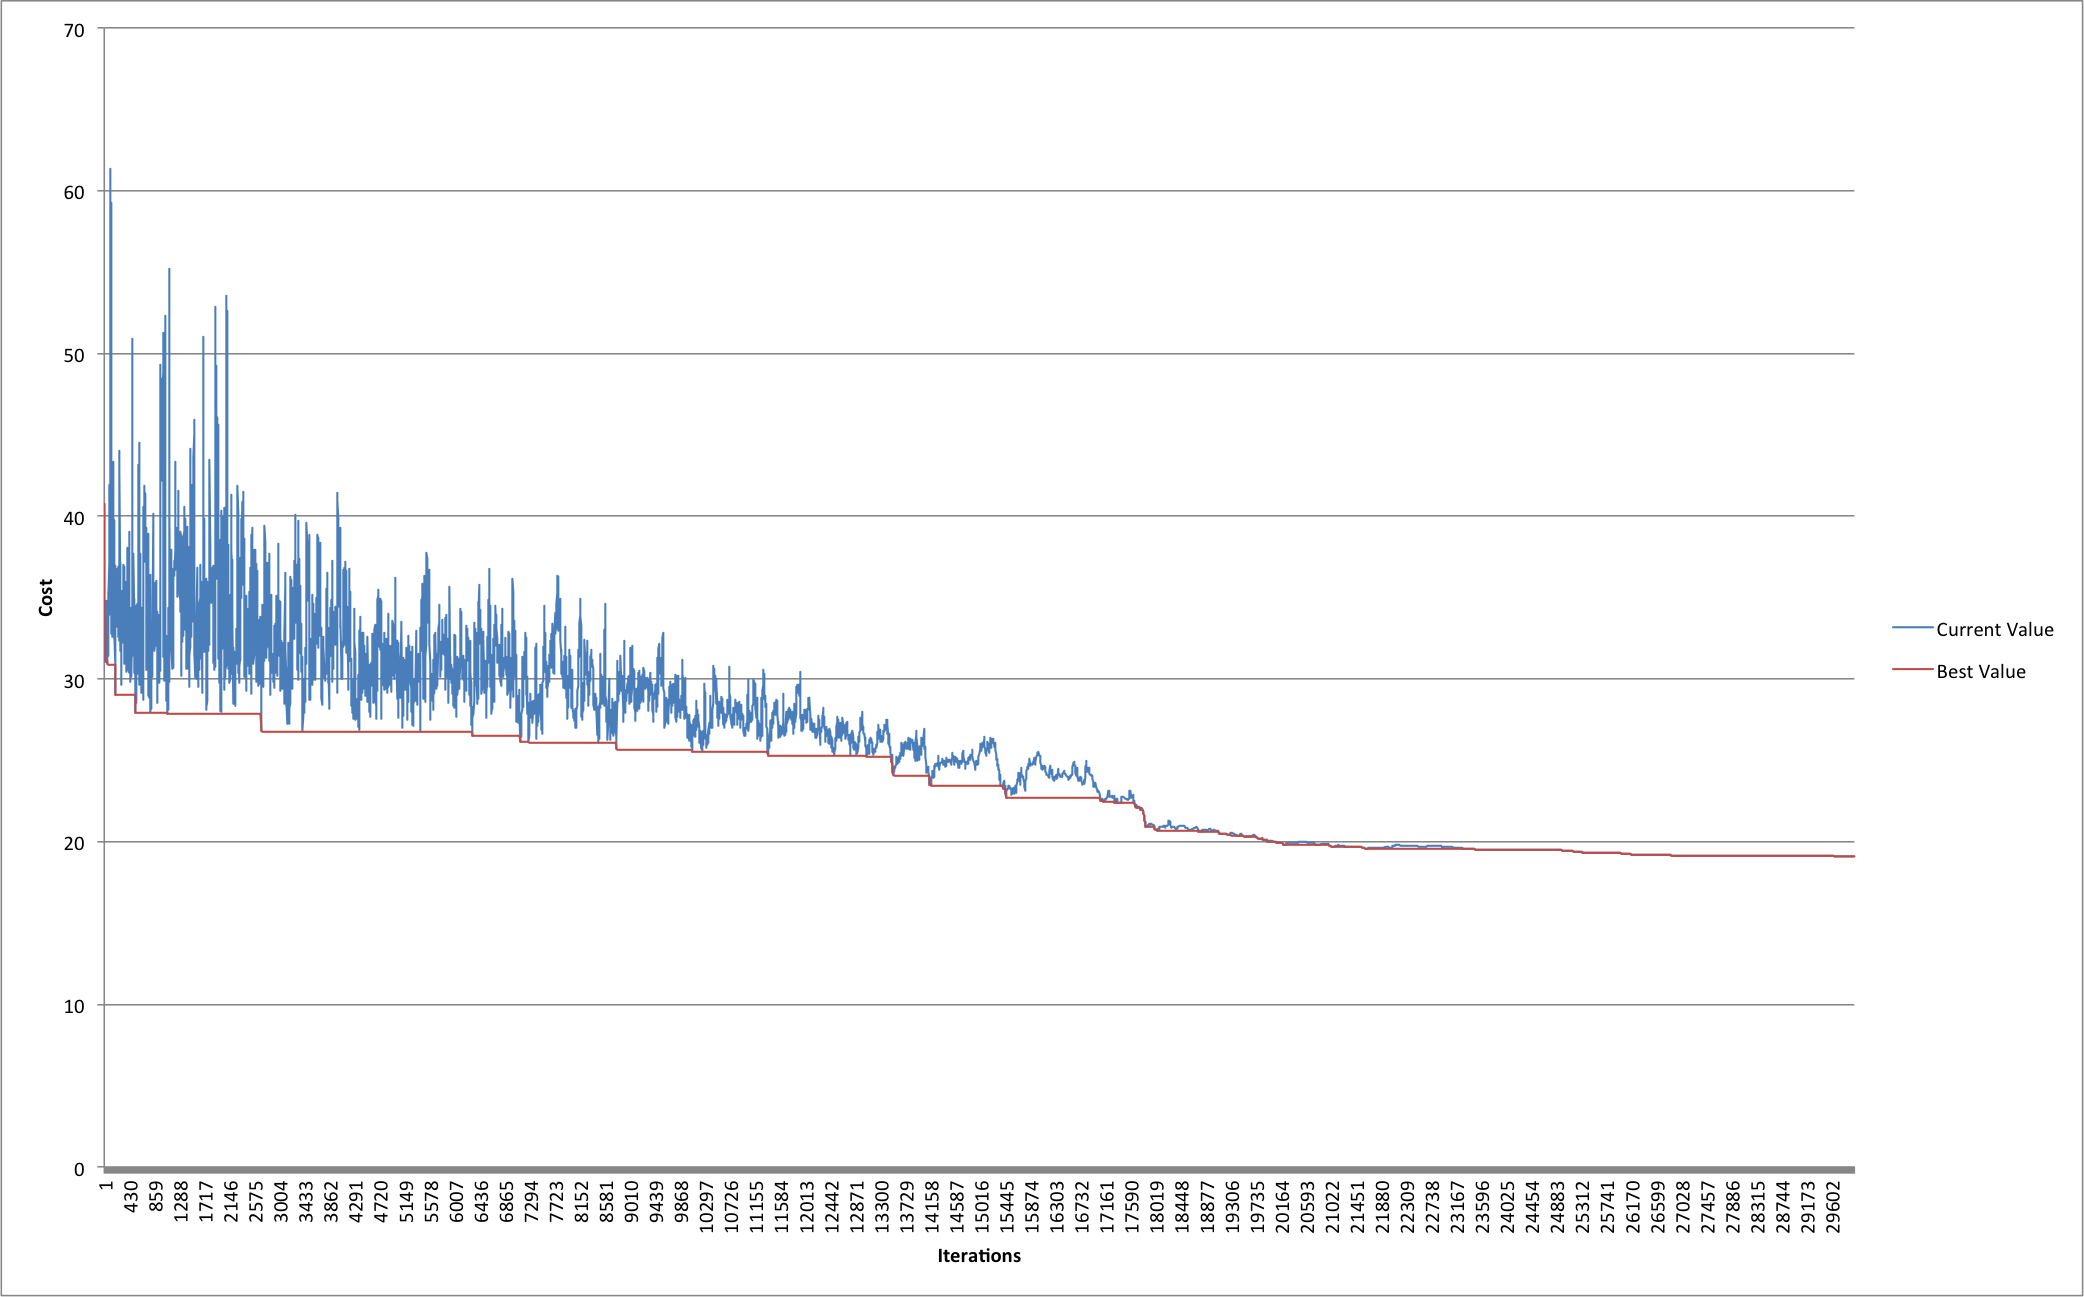
\includegraphics[width=1.2\textwidth]{images/SAplot.png}
}
\caption{Simulated Annealing run on large data set}
\end{figure}
\end{center}

\subsubsection{Hand Iterations}

In these hand iterations, a geometric cooling schedule will be used with an initial temperature $T_0 = 3$ and cooling factor $\alpha_\mathit{cooling} = 0.8$
$$T_i = T_0 \cdot \left( \alpha_\mathit{cooling} \right)^{i - 1}$$

\subsubsubsection{Iteration 1}

We begin with our randomly selected initial solution
$$S_\mathit{best} = S_0 = [ 1, 2, 0, 3 ], \; \mathit{cost}(S_0) = 3.1617$$
and swap two randomly selected elements (4 and 3) to create a neighboring
solution, $S_1$
$$S_1 = [ 1, 2, 3, 0 ], \; \mathit{cost}(S_1) = 4.3288$$

To decide whether or not $S_1$ should become $S_\mathit{next}$, we calculate its
selection probability, $P_1$, as
\begin{align*}
P_i & =
\begin{cases}
  1 & \mathit{cost}(S_{i}) < \mathit{cost}(S_{i - 1}) \\
  \exp \left\{-\frac{\mathit{cost}(S_{i}) - \mathit{cost}(S_{i - 1})}{T_i}\right\} & \text{otherwise}
\end{cases} \\
P_1 & = 0.6777
\end{align*}

$S_1$ becomes $S_\mathit{next}$ if and only if a randomly selected number,
$r \in [0, 1]$, makes the inequality $r < P_1$ true.

Suppose we choose $r = 0.3597$. Because $0.3597 < 0.6777$
$$S_\mathit{next} = S_1 = [ 1, 2, 3, 0 ], \; \mathit{cost}(S_\mathit{next}) = 4.3288$$

\subsubsubsection{Iteration 2}

We begin by swapping two randomly selected elements (1 and 3) in $S_\mathit{next}$
$$S_2 = [ 3, 2, 1, 0 ], \; \mathit{cost}(S_2) = 4.6092$$

We calculate this solution's selection probability to be $P_2 = 0.8897$

Suppose we choose $r = 0.6329$. Because $0.6329 < 0.8897$ is true
$$S_\mathit{next} = S_2 = [ 3, 2, 1, 0 ], \; \mathit{cost}(S_\mathit{next}) = 4.6092$$

The best solution found so far is
$$S_\mathit{best} = [ 1, 2, 0, 3 ], \; \mathit{cost}(S_\mathit{best}) = 3.1617$$

\subsubsection{Parameter Tuning}

When tuning simulated annealing, there seems to be an optimal temperature range in which the most improvements towards the best solution are found. If the temperature is too high, there will be too much exploration for the algorithm to make meaningful progress. However, should the temperature be too low, the algorithm will get stuck in local optima.

For geometric cooling, using a higher cooling factor seems to produce better results at the expense of requiring more iterations. A higher cooling factor means that more temperature values will be used, so the algorithm will spend more time in the optimal temperature range. Conversely, a lower cooling factor appears to be more effective for a linear cooling schedule.

More iterations per temperature can be used to increase the exploitation at each temperature, producing better results at the expense of significantly more computation time. After a certain point, adding more iterations per temperature does not improve the solutions found.

Appropriate initial and minimum temperature values are quite similar between data sets, as the cooling factor and iterations per temperature parameters are more useful in controlling the total number of iterations. If the maximum temperature is too high, the algorithm wastes time at the start by exploring too much. Setting the minimum temperature too low causes the geometric cooling algorithm to run for significantly more iterations with little benefit, being much more likely to get stuck in local optima. The minimum temperature has less of an effect when linear cooling is used, but is still necessary to prevent the algorithm from getting stuck in local optima.

On the small data set, geometric cooling seems to find the optimal solution more reliably than linear cooling. On the medium data set, geometric cooling seems to find better solutions in fewer iterations. On the large data set, linear seems to perform similarly to geometric.

\todo{reference data sets in the appendix}

\subsection{Genetic Algorithm} % Austin

Genetic Algorithm(GA) is a class of algorithms that use techniques from natural selection and biology in order to solve optimization problems. The basic idea of GA is to simulate a population of animals that breed and experience selection pressure to evolve to the optimal solution. The population is modified according to methods that are taken from nature including sexual recombination and mutation. Sexual recombination is modeled by crossover functions and mutation is modeled by mutation functions.

Genetic algorithms cover a large group of similar algorithms, so for our comparative study it is necessary to specify an instance of Genetic Algorithm that solves the problem adequately.

Since this is a permutation problem we are unable to encode the solution as a binary string; thus it is necessary to use a version of Genetic Algorithm which can handle permutations.

To initialize the solver we choose a random starting solution for each individual and then start iterating. Each iteration will consist of crossover, mutation and then survivor selection, each step of which must be customized for the problem set. Each step has many alternatives between which it is necessary to choose.

For crossover we chose to use the Order 1 permutation as described in \cite{Eiben} -- a crossover algorithm that attempts to preserve the relative order of elements in a solution. It chooses a random subsection from one parent, copies those values into the first child and then fills the rest of the values in the same order that they appear in the second parent. This process is then mirrored for the second child so two children are produced from this crossover.

The mutation function is much easier to specify in a permutation problem, because there are fewer issues relating to creating invalid solutions -- a large issue when attempting to do crossover. Mutation in our algorithm swaps the position of two or more elements in a solution and then creates a new child. The number of elements swapped can be configured depending on the size of the solution.

The last component that needs to be specified is the survivor selection algorithm. We chose to use a steady state Genetic Algorithm, considering the entire generation and the children when choosing the new population. We use an elitism-based selection method which causes our new generations to only contain the best members from the previous generation \cite{Talk}. This method was chosen because it caused the algorithm to converge faster to optimal values.

With our algorithm specified fully we can now do iterations by hand to see the results of our decisions.

\subsubsection{Hand Iterations}

The genetic algorithm metaheuristic has many different parameters that can be tuned and changed, but for the hand iteration we will choose values that show the different operations of the algorithm. We will use a generation size of 4 and choose $p_\mathit{crossover}=0.75$, and $p_\mathit{mutation}=0.25$ because $p_\mathit{mutation}$ must be between $$\frac{1}{\text{Population Size}} <= p_\mathit{mutation} < \frac{1}{\text{Chromosome Length}}$$ For every child, a random number, $r \in (0,1)$, will be generated. If $0<r\leq0.25$ then mutation will be applied, else if $0.25<r<1$ then crossover will be applied.

This is a permutation problem, so we will use the Order 1 crossover algorithm. We also choose the mutation operator to be a swap operation that swaps two elements in a solution.

\subsubsubsection{Iteration 1}

We generate 4 random solutions to be members of the first generation.

\begin{align*}
S_{0,1} = [1, 2, 0, 3], & \qquad cost(S_{0,1}) = 3.1617 \\
S_{0,2} = [3, 2, 0, 1], & \qquad cost(S_{0,2}) = 3.6619 \\
S_{0,3} = [2, 0, 1, 3], & \qquad cost(S_{0,3}) = 2.9759 \\
S_{0,4} = [3, 2, 1, 0], & \qquad cost(S_{0,4}) = 4.6092
\end{align*}

We now generate a random number to see if crossover or mutation will produce the first child(ren). $r=0.37$ so we will use crossover.

We will perform the crossover by choosing two random parents, $S_{0,1}$ and $S_{0,3}$. We apply Order 1 crossover, with the two crossover points as 1 and 2. The two children will be:

\begin{align*}
S_{1,1} = [1, 2, 3, 0], & \qquad cost(S_{1,1}) = 4.3288 \\
S_{1,2} = [2, 0, 3, 1], & \qquad cost(S_{1,2}) = 3.0201
\end{align*}


Another random number is genereated: $r=0.65$, another crossover. This crossover will be between $S_{0,2}$ and $S_{0,4}$, with crossover points as 2 and 4. This yields two more children:

\begin{align*}
S_{1,3} = [3, 2, 0, 1], & \qquad cost(S_{1,3}) = 3.6619 \\
S_{1,4} = [3, 2, 1, 0], & \qquad cost(S_{1,4}) = 4.6092
\end{align*}


The next generation is selected using the cost based elitism survivor selection; we will pick the best 4 solutions from the 8 candidates. The result of this selection is:

\begin{align*}
S_{1,1} = [1, 2, 0, 3], & \qquad cost(S_{1,1}) = 3.1617 \\
S_{1,2} = [2, 0, 3, 1], & \qquad cost(S_{1,2}) = 3.0201 \\
S_{1,3} = [2, 0, 1, 3], & \qquad cost(S_{1,3}) = 2.9759 \\
S_{1,4} = [3, 2, 0, 1], & \qquad cost(S_{1,4}) = 3.6619
\end{align*}

\subsubsubsection{Iteration 2}
A random number is generated: $r=0.89$, a crossover. This crossover will be between parents $S_{1,1}$ and $S_{1,2}$ and use crossover points 3 and 4.

\begin{align*}
S_{2,1} = [2, 1, 0, 3], & \qquad cost(S_{2,1}) = 3.8583 \\
S_{2,2} = [2, 0, 3, 1], & \qquad cost(S_{2,2}) = 3.0201
\end{align*}

The next random number is: $r=0.18$, a mutation. We will mutate one randomly chosen parent, $S_{1,2}$, by swapping the randomly chosen indicies 3 and 4.

\begin{align*}
S_{2,3} = [2, 1, 3, 0], & \qquad cost(S_{2,3}) = 4.6371
\end{align*}

The next random number is: $r=0.05$, a mutation. We will mutate one randomly chosen parent, $S_{1,4}$ by swapping the randomly chosen indicies 1 and 2.

\begin{align*}
S_{2,4} = [2, 3, 0, 1], & \qquad cost(S_{2,4}) = 4.0781
\end{align*}

Again, cost-based elitism survivor selection is used to pick the best 4 solutions from both generations. We are left with the same generation as the last iteration because none of the children had a higher fitness score than any of the parents.

\begin{align*}
S_{2,1} = [1, 2, 0, 3], & \qquad cost(S_{2,1}) = 3.1617 \\
S_{2,2} = [2, 0, 3, 1], & \qquad cost(S_{2,2}) = 3.0201 \\
S_{2,3} = [2, 0, 1, 3], & \qquad cost(S_{2,3}) = 2.9759 \\
S_{2,4} = [3, 2, 0, 1], & \qquad cost(S_{2,4}) = 3.6619
\end{align*}

\subsubsection{Parameter Tuning}

Genetic Algorithm is a complex algorithm with many different parameters needing specification, so after initially creating our solution we made many modifications to our initial algorithm parameters.

One of the initial parameters we could tune are the crossover and mutation probabilities. The crossover probability did not seem to be a huge factor in convergence, values from $.6$ - $.95$ would all converge to the same values with relative ease.

The mutation probability was chosen to be in the range $$\frac{1}{\text{Population Size}} <= p_\mathit{mutation} < \frac{1}{\text{Chromosome Length}}$$ and the mutation sites variable was modified so as many as $\frac{\text{Chromosome Length}}{2}$ swaps were performed when a mutation needed to be performed.

The other modification we made after initially developing our algorithm was to change our stopping criteria from a strict number of iterations to a criterion by which we detect stagnation in the best solution and stop only then. This helps to fully explore the solution space and allows us to fairly compare this algorithm against our others.

Due to the large number of parameters we have to tune, the most efficient method to discover a good configuration would be to make an adaptive version of this algorithm to tune the parameters based on running itself recursively, though this would still not give us the best possible configuration.

This solution to tuning would still not be optimal since it would also need a way to change its crossover, mutation and survivor-selection algorithms. Each of these sub-algorithms has multiple different implementations.

\subsection{Particle Swarm Optimization Algorithm}
% Ariel
The particle Swarm Optimization (PSO) metaheuristic is based on the behavior of swarm animals such as fish and birds.

Each particle represents a candidate solution and ``flies'' towards the optimal solution using information from it and the swarm's collective experience. Gradually, these particles will converge on the optimal solution.

This algorithm begins by generating an initial population of particles, each of which has a velocity of 0.

In each iteration, the local (per particle) and global (across the swarm) best values are recorded and used to calculate each particle's new velocity \cite{ClassicalPSO} as:
$$
v_\mathit{next} = wv_\mathit{current} + c_1r_1(l_\mathit{best} - x) + c_2r_2(g_\mathit{best}-x)
$$

where $w$ is a constant representing a particle's inertia and $c_1, c_2$ are two pre-selected parameters to adjust the relative importance of a particle's individual memory versus the swarm's collective memory.

The variables $r_1$ \& $r_2$ are random numbers $\in (0,1)$ that are generated on a per-iteration basis. $l_\mathit{best}$ is the best position in which a particle has found itself and $g_\mathit{best}$ is likewise defined for the swam collective.

The overall algorithm can be visualized as follows \cite{PSOFigure}:

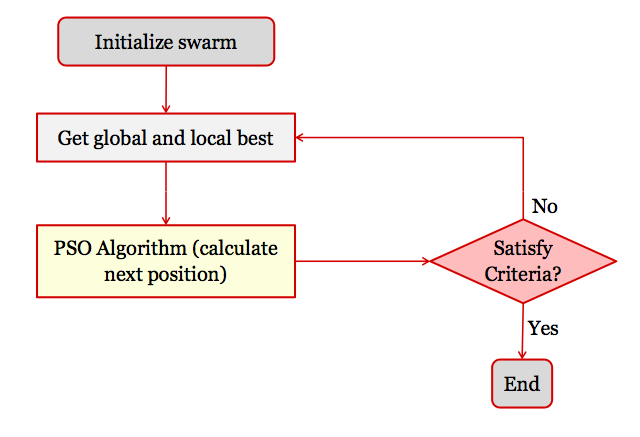
\includegraphics[width=1\textwidth]{images/PSO.png}

where satisfy criteria is defined in this report as performing a specified number of iterations.\\

mTSP is a permutation problem and therefore this report necessarily makes some modifications to the classic PSO algorithm:

The difficulty arises from the fact that position and velocity do not have a natural meaning when working
with permutations. However, Clerc\cite{PermutationPSO} proposed a modification of PSO that can be applied to TSP:

Every particle's position is a candidate solution which is a permutation of tasks and homes and
a particle's velocity consists of a set of swaps that should be performed on its position.

Clerc then redefines the operations of position/velocity addition, position subtraction and scalar multiplication:
\begin{itemize}
\item Adding a velocity to a position is defined as performing all of the swaps on the position.
\item Multiplying a velocity by a scalar results in a new velocity that consists of $scalar\cdot |velocity|$ swaps; which is achieved through truncation or augmentation with swaps repeated from the existing velocity.
\item Subtracting two positions results in a velocity that consists of the swaps needed to turn the first position into the second position.
\end{itemize}
Given these new operations, the classical PSO algorithm can be used as-is.

Another consideration has been made to adapt to the issue of stagnation. After failure to find a more-optimal solution in 15 iterations, the particles are ``scattered'': they are all assigned random new positions and half of them retain the swarm's ``memory''. That is to say that half of the particles have an $l_\mathit{best}$ equal to the most optimal solution found by the swarm so far and the other half simply have an $l_\mathit{best}$ set to their new current position.

This strikes a balance between exploitation of the previous best solution and exploration of new spaces.

\subsubsection{Hand Iterations}

\todo{don't say \"in this course\", find the actual citation.}
As per the recommendations in this course, we set the following constants
\begin{align*}
c_1 = c_2 & = 1.4944 \\
w & = 0.792
\end{align*}

\subsubsubsection{Iteration 1}

Let $r_1 = 0.7426$ and $r_2 = 0.4276$ as random constants for this iteration.

We start with three randomly selected initial positions (solutions)
\begin{align*}
S_{1,1} = [1, 2, 0, 3], & \; cost(S_{1,1}) = 3.1617 \\
S_{1,2} = [3, 2, 0, 1], & \; cost(S_{1,2}) = 3.6619 \\
S_{1,3} = [1, 0, 3, 2], & \; cost(S_{1,3}) = 3.6494
\end{align*}

Observe that $S_{1,1}$ has the lowest initial score. This becomes our initial $S_\mathit{gbest}$.
$$S_\mathit{gbest} = [1, 2, 0, 3], \; cost(S_\mathit{gbest}) = 3.1617$$

For this algorithm, we track not only the best solution seen globally,
$S_\mathit{gbest}$, but the best solution seen by each particle, $i$, as
$S_{\mathit{lbest}, i}$.

For each position, $i$, we calculate
$v_{1,i}$ using the following equation. Note that we redefine the subtraction of
two positions, the addition of a velocity and a position, and the multiplication
of a velocity by a scalar as defined above\cite{DiscretePSO}.\todo{This citation doesn't exist}
$$
v_{j,i} =
  w v_{j-1, i} +
  c_1 r_1 (S_{\mathit{lbest}, i} - S_{j-1, i}) +
  c_2 r_2 (S_\mathit{gbest} - S_{j-1, i})
$$

\begin{center}
\begin{tabular}{lllllll}
          & \textbf{position} & \textbf{cost} & \textbf{lbest position} & \textbf{lbest cost} & $v_1$ & $v_2$            \\
$S_{1,1}$ & $[1, 2, 0, 3]$    & $3.1617$      & $[1, 2, 0, 3]$          & $3.1617$            & $[]$  & $[]      $ \\
$S_{1,2}$ & $[3, 2, 0, 1]$    & $3.6619$      & $[3, 2, 0, 1]$          & $3.6619$            & $[]$  & $[(1, 4)]$ \\
$S_{1,3}$ & $[1, 0, 3, 2]$    & $3.6494$      & $[1, 0, 3, 2]$          & $3.6494$            & $[]$  & $[(2, 4)]$ \\
\end{tabular}
\end{center}
\vspace{1.5em}

\subsubsubsection{Iteration 2}

We choose $r_1 = 0.2351$ and $r_2 = 0.8262$ as random constants for this
iteration.

Applying the $v_2$ velocities calculated in iteration 1 to the positions in
iteration 1, we obtain the positions for iteration 2 and calculate new
velocities accordingly
\begin{center}
\begin{tabular}{lllllll}
          & \textbf{position} & \textbf{cost} & \textbf{lbest position} & \textbf{lbest cost} & $v_1$      & $v_2$            \\
$S_{2,1}$ & $[1, 2, 0, 3]$    & $3.1617$      & $[1, 2, 0, 3]$          & $3.1617$            & $[]      $ & $[]$             \\
$S_{2,2}$ & $[1, 2, 0, 3]$    & $3.1617$      & $[1, 2, 0, 3]$          & $3.1617$            & $[(1, 4)]$ & $[]$             \\
$S_{2,3}$ & $[1, 2, 3, 0]$    & $4.3288$      & $[1, 0, 3, 2]$          & $3.6494$            & $[(2, 4)]$ & $[(3,4), (3,4)]$ \\
\end{tabular}
\end{center}
\vspace{1.5em}

After two iterations, we have
$$S_\mathit{gbest} = [1, 2, 0, 3], \; cost(S_\mathit{gbest}) = 3.1617$$

\subsubsection{Parameter Tuning}
Particle Swarm Optimization has four main parameters to be tuned:

$w$ is the inertia factor that determines how much of a particle's velocity is retained between iterations. $c_1, c_2$ which control the relative importance of an individual's memory versus that of the swarm, respectively. $n_{particles}$ is the number of particles used for simulation.\\

Through empirical testing, it became apparent that a velocity did not retain any meaningful notion of direction between iterations. A set of swaps has a completely different impact depending on what position it is applied to. For this reason, $w$ was set to 0.

To compensate for the lack of inertia, $c_1$ \& $c_2$ have two values:

$$
c_1 =
\begin{cases}
1.4 & \text{if } \mathit{cost}(l_\mathit{best}) \leq \mathit{cost}(g_\mathit{best})\\
0.25 & \text{if } \mathit{cost}(g_\mathit{best}) > \mathit{cost}(l_\mathit{best})
\end{cases}
$$

$$
c_2 =
\begin{cases}
0.25 & \text{if } \mathit{cost}(l_\mathit{best}) \leq \mathit{cost}(g_\mathit{best})\\
1.4 & \text{if } \mathit{cost}(g_\mathit{best}) > \mathit{cost}(l_\mathit{best})
\end{cases}
$$

This allows the best solution to be ``chased'' directly by a particle while still introducing an amount of exploration from the less desirable input. It is unknowable in advance whether $c_1$ should be different and empirical evidence did not suggest that any benefit in having them take on different values. \cite{PermutationPSO}\\

Finally, the swarm size was tuned experimentally, due to there being nothing but rough heuristics on its assignment The number of particles used was correlated with the number of variables in the candidate solution for a given instance of MRTA. \cite{PermutationPSO}

\subsection{Ant Colony Optimization Algorithm} % Sandy

We use a variation of ACS to solve this instance of complex task allocation as follows:

Let us define the pheromone evaporation constant $\rho=0.7$.\\
The desirability function is defined by:

\begin{equation*}
\resizebox{0.9\textwidth}{!}{$
\mathit{d}(r, t_\mathit{from}, t_\mathit{to}) = \begin{cases}
  0 & \text{if } t_\mathit{to} = \mathit{home}(robot) \\
  \left(
  (1 - \alpha)
    (\mathit{priority}(t_\mathit{to}) \mathit{skill}(r, t_\mathit{to})) +
    \alpha \beta
    \mathit{e}_{cost}(t_\mathit{from}, t_\mathit{to})
  \right)^{-1}
  & \text{if }\mathit{accomplishable}(r, t_\mathit{from}, t_\mathit{to}) \\
  - \infty
  & \text{otherwise} \\
\end{cases}
$}
\end{equation*}
where $\mathit{accomplishable}$ is defined as:
$$
\mathit{accomplishable}(r, t_\mathit{from}, t_\mathit{to}) =
\frac{\mathit{round\,trip}(r, t_\mathit{from}, t_\mathit{to})}{velocity(r)} + \mathit{task \, time}(r, t_\mathit{to}) \leq \mathit{energy}_r
$$
for:
$$
\mathit{round\,trip}(r, t_\mathit{from}, t_\mathit{to}) = \mathit{distance}(t_\mathit{from}, t_\mathit{to}) + \begin{cases}
\mathit{distance}(t_\mathit{to}, \mathit{home}(r)) & \text{if } t_\mathit{to} \ne \mathit{home}(r) \\
0 & \text{otherwise}
\end{cases}
$$

We then define an $r_0$ value that will be used to control the level of exploitation versus the level of exploration by the ants.
For each state transition the ant makes, a random number, $r$, is generated.
If $r\leq r_0$ then the most desirable path (weighted by pheromones) is exploited, else if $r>r_0$
a randomly selected path is explored. We will use a value of $r_0=0.43$.

The most desirable path is defined as the neighboring node that maximizes:
$$
\tau_{iu}\eta_{iu}^\beta
$$
where $i$ represents the current node of the ant and $u$ is a neighboring node.

For exploration, random path selection is done via the Roulette Wheel Method.
Probabilities are generated by:
$$
p_{ij}=
\begin{cases}
\frac{\tau_{ij}\eta_{ij}^\beta}{\sum\limits_{u\in N_i} \tau_{iu}\eta_{iu}^\beta} & \text{if } j \in N_i\\
0 & \text{if } j \not\in N_i
\end{cases}
$$
with $N_i$ representing the neighbors of node $i$.

The most important modification to ACS is how the sentinel values of a canonical solution vector $S$ are handled.
The key insight for this change is a subtle modification of the graph during search-time. Define the distance between any
two $home$s to be 0, and, at first, connect each task node only to $home(1)$.

Upon returning to $\mathit{home}(1)$, ``teleport'' the ant to $\mathit{home}(2)$, connecting it to all
of the task nodes, and disconnecting the tasks from $\mathit{home}(1)$. In effect, we are swapping the node associated with $\mathit{home}(1)$ out with the node $\mathit{home}(2)$. Upon doing this, update an
internal state variable $robot_{current}$, whose purpose it is to correctly
evaluate the $d()$ function.

The first two iterations of performing ACS on the reduced problem are shown below:

\subsubsection{Iteration 1}

The starting node is $\mathit{home}(1) = 4$, with parameters $\alpha = \beta = 1, \rho = 0.7, r_0 = 0.5$.

\subsubsubsection{Ant Travel}

We first compute the cumulative desirability $\eta$ of this node's neighbors, used to normalize the relative desirabilities later.

$$
\eta = \sum_{n \in N_4} \uptau_{4n}^\alpha d_{4n}^\beta = 6.2913
$$

We then proceed to compute the relative probabilities of traveling to any given node as follows, with the bold probability being the edge chosen by the Roulette Wheel Method:

\begin{align*}
p_{4i} &= \frac{\uptau_{4n}^\alpha d_{4i}^{-\beta}}{\eta} \\
\\
p_{41} &= 0.26070 \\
\mathbf{p_{42}} &= \mathbf{0.25154} \\
p_{43} &= 0.24933 \\
p_{44} &= 0.23842
\end{align*}

This corresponds to the partially constructed canonical vector solution and energy of $robot_1$:

$$
S(1) = \{4, 2\} \qquad \mathit{energy}(1) = 40.096
$$

% % %

Repeat the above steps for the newly selected node 2:

$$
\eta = \sum_{n \in N_2} \uptau_{2n}^\alpha d_{2n}^\beta = 4.5890
$$

\begin{align*}
p_{2i} &= \frac{\uptau_{2n}^\alpha d_{2i}^{-\beta}}{\eta} \\
\\
\mathbf{p_{21}} &= \mathbf{0.34080} \\
p_{23} &= 0.33233 \\
p_{24} &= 0.32687
\end{align*}

$$
S(1) = \{4, 2, 1\} \qquad \mathit{energy}(1) = 28.742
$$

and again:

$$
\eta = \sum_{n \in N_1\setminus\{2\}} \uptau_{1n}^\alpha d_{1n}^\beta = 3.0489
$$

\begin{align*}
p_{1i} &= \frac{\uptau_{1n}^\alpha d_{1i}^{-\beta}}{\eta} \\
\\
\mathbf{p_{13}} &= \mathbf{0.50802} \\
p_{14} &= 0.49198 \\
\end{align*}

$$
S = \{2, 1, 3, 0\} \qquad \mathit{energy}(1) = 6.4352 \qquad d_{tour} = 6.1953
$$

Note that traveling to $\textit{home}(1) = 4$ has triggered the ant to automatically move to $\textit{home}(2) = 5$, and thus the ant now uses $robot_2$'s cost function.

\subsubsubsection{Update Pheromone Trail}

First, we decay the pheromone matrix by $1-\rho$:
$$
\uptau = (1 - \rho)\uptau =
\begin{tabular}{r | c c c c c}
$i \setminus j$ & 1 & 2 & 3 & 4 & 5 \\
\hline
1 & 0.30000 & 0.30000 & 0.30000 & 0.30000 & 0.30000 \\
2 & 0.30000 & 0.30000 & 0.30000 & 0.30000 & 0.30000 \\
3 & 0.30000 & 0.30000 & 0.30000 & 0.30000 & 0.30000 \\
4 & 0.30000 & 0.30000 & 0.30000 & 0.30000 & 0.30000 \\
5 & 0.30000 & 0.30000 & 0.30000 & 0.30000 & 0.30000
\end{tabular}
$$

and proceed to update the pheromone matrix with the constant $Q/d_{tour}$ -- in effect the ant returns home via the same path, laying pheromone over the entire distance:

$$
\uptau_{ij} = \uptau_{ij} + Q/\mathit{cost}(S) =
\begin{tabular}{r | c c c c c}
$i \setminus j$ & 1 & 2 & 3 & 4 & 5 \\
\hline
1 & 0.30000 & 0.30000 & 0.51565 & 0.30000 & 0.30000 \\
2 & 0.51565 & 0.30000 & 0.30000 & 0.30000 & 0.30000 \\
3 & 0.30000 & 0.30000 & 0.30000 & 0.51565 & 0.30000 \\
4 & 0.30000 & 0.51565 & 0.30000 & 0.30000 & 0.51565 \\
5 & 0.30000 & 0.30000 & 0.30000 & 0.30000 & 0.51565
\end{tabular}
$$



\subsubsection{Iteration 2}

The second iteration proceeds entirely as above:

\subsubsubsection{Ant Travel}
$$
\eta = \sum_{n \in N_4} \uptau_{4n}^\alpha d_{4n}^\beta = 2.2287
$$

\begin{align*}
p_{4i} &= \frac{\uptau_{4n}^\alpha d_{4i}^{-\beta}}{\eta} \\
\\
p_{41} &= 0.22078 \\
p_{42} &= 0.36615 \\
\mathbf{p_{43}} &= \mathbf{0.21115} \\
p_{44} &= 0.20192
\end{align*}

$$
S(1) = \{4, 3\} \qquad \mathit{energy}(1) = 47.028
$$

% % %

$$
r < r_0 \to \text{automatically choose most desirable path, 4}
$$

$$
S(1) = \{4, 3, 4\} \qquad \mathit{energy}(1) = 37.704
$$

Note that because node 4 was visited, 5 was also visited and now $robot_{current} = 2$.

% % %

$$
\eta = \sum_{n \in N_5\setminus\{3\}} \uptau_{2n}^\alpha d_{5n}^\beta = 1.0070
$$

\begin{align*}
p_{3i} &= \frac{\uptau_{2n}^\alpha d_{1i}^{-\beta}}{\eta} \\
\\
p_{31} &= 0.50890 \\
\mathbf{p_{32}} &= \mathbf{0.49110}
\end{align*}

$$
S(2) = \{5, 2, 1\} \qquad \mathit{energy}(2) = 13.132 \qquad d_{tour} = 3.2795
$$

Node 1 was automatically selected since after choosing 2, it was all that remained.

\subsubsubsection{Update Pheromone}

$$
\uptau = (1 - \rho)\uptau =
\begin{tabular}{r | c c c c c}
$i \setminus j$ & 1 & 2 & 3 & 4 & 5 \\
\hline
1 & 0.090000 & 0.090000 & 0.154696 & 0.090000 & 0.090000 \\
2 & 0.154696 & 0.090000 & 0.090000 & 0.090000 & 0.090000 \\
3 & 0.090000 & 0.090000 & 0.090000 & 0.154696 & 0.090000 \\
4 & 0.090000 & 0.154696 & 0.090000 & 0.090000 & 0.154696 \\
5 & 0.090000 & 0.090000 & 0.090000 & 0.090000 & 0.154696
\end{tabular}
$$

$$
\uptau_{ij} = \uptau_{ij} + Q/\mathit{cost}(S) =
\begin{tabular}{r | c c c c c}
$i \setminus j$ & 1 & 2 & 3 & 4 & 5 \\
\hline
1 & 0.090000 & 0.090000 & 0.154696 & 0.090000 & 0.355319 \\
2 & 0.420015 & 0.090000 & 0.090000 & 0.090000 & 0.090000 \\
3 & 0.090000 & 0.090000 & 0.090000 & 0.420015 & 0.090000 \\
4 & 0.090000 & 0.154696 & 0.355319 & 0.090000 & 0.420015 \\
5 & 0.090000 & 0.355319 & 0.090000 & 0.090000 & 0.154696
\end{tabular}
$$

\subsubsubsection{Result}

To determine the result, we look through all solutions created by the ants earlier, and return the one with the highest total desirability.

$$
S = \{1, 2, 0, 3\} \qquad d_{best} = 0.8900
$$


\subsubsection{Parameter Tuning}

Our ACO implementation had four parameters (separate from our cost function) needing to be tuned, $\alpha, \beta, \rho, r_0$, the exploitation constant, exploration constant, pheromone evaporation rate and likelihood-of-exploitation probability, respectively. These parameters form a \todo{I like burritos, but...} burrito-optimality frontier, where none can be changed without negatively impacting the entire system, however, such a burrito-optimal solution is not unique. In addition, several regions of the parameter space prevented convergence entirely.

The initial search strategy of this parameter space was conducted entirely randomly -- we generated 100 sets of random values for each parameter in the range of $\alpha, \rho, r_0 \in [0, 1], \beta \in [1, 2]$, and performed ten searches on the small data set to find the average case. If any set of parameters failed to converge in 20 iterations, it was immediately thrown out.

We selected the parameter set which corresponded to the best average solution case and hand-tuned each variable sequentially to the nearest hundredth. Surprisingly, when mapping our new parameters to the larger problem sets, no amount of further hand-tuning was capable of finding a better solution in either domain. Thus, we consider the parameters $\alpha = 0.41, \beta = 1.15, \rho = 0.76, r_0 = 0.43$ to be burrito-optimal for the purposes of complex task allocation with ACO.

However, despite being unable to come up with better solutions when tweaking the parameters, ACO's solutions for the large data set were qualitatively poor. Most solutions it converged to were obvious local optima; almost all of them were worse than 1.5x the best located solution by other metaheuristics. We spent over 4 person-hours attempting to tweak these parameters to no avail. While researching this, it was noted that reseting the pheromone trail to a random solution after each iteration would perform better than maintaining it, implying our desirability function was non-reflexive.

\newpage
\section{Performance Evaluation}

Each metaheuristic will be evaluated quantitatively and qualitatively.

The following instances of MRTA will be studied:
\begin{enumerate}
\item \textbf{Small scale}: Five tasks and three robots
\item \textbf{Medium scale}: Fifteen tasks and five robots
\item \textbf{Large scale}: Fifty tasks and fifteen robots
\end{enumerate}

The different scenarios will allow for qualitative analysis on the scalability of metaheuristic techniques and where they are best applied. Within each scenario, each technique can be compared using some quantitative metrics. Badreldin et al. \cite{Badreldin} identify two suitable measures: the computational time taken to find the best solution and the optimality of the best solution obtained by a metaheuristic technique.

Our experimental data was generated randomly because there are no canonical data sets for the MRTA problem that we could find. For each of the data sets there were 6 different parameters generated randomly: a $\mathit{priority(task)}$ vector, a $\mathit{distance(node, node)}$ matrix, a $\mathit{skill(robot, task)}$ matrix, a $\mathit{task\,time(robot, task)}$ matrix, an $\mathit{energy(robot)}$ matrix and a $\mathit{velocity(robot)}$ vector.

The experiment run was to evaluate each algorithms five times over each dataset. The algorithms were run on a single MacBook Pro with a 2.3GHz quad-core Intel Core-i7 processor, and 16GB of RAM to ensure numeric consistency between the individual optimization processes.

Each algorithm created a .csv file with a standardized output in an attempt to run identical analyses throughout. Such a system facilitated easy creation of graphs and other statistical tools. The analysis under discussion revealed some interesting results when compared over quantitative metrics.

Our results revealed that each algorithm had both defining properties and a distinct performance profile. For example, the TS algorithm converged most quickly to a reasonable solution, but failed to find optimal solutions in most cases. Simulated Annealing converged more slowly, but resulted in the best solutions of the algorithms compared by this report.

The other algorithms were suboptimal in either speed or optimality of solution, though they did have some positive performance characteristics. The GA implementation consistently found good solutions, but was found to converge very slowly. PSO and ACO both solved the smaller problem sets in record time, but neither performed well on the large dataset. 

\subsection{Small Scale}

Our small dataset problem featured a very small permutation space with $8! = 40320$ possibilities, on which most of our metaheuristic algorithms were able to converge to the same solution. We take this as strong evidence of having found the optimal solution (though recall this is not a canonical dataset, so we are uncertain in this claim).

The problem displays some of the differences between the algorithms, with both TS and SA being very effective with fast convergence to the optimal solution. GA, ACO and PSO also converged to the optimal value, but more slowly than TS and SA. This is a property that we will see in the larger datasets where said differences are more pronounced.

\subsection{Medium Scale}

The results for the medium scale data set were similar to the results from the small scale data set. All of the algorithms were able to converge and find a reasonable solution for this problem. In this data set we can see that the P-Metaheuristic algorithms still had trouble converging quickly because their iteration times are much larger than the iteration times for the S-Metaheuristic algorithms. 

\subsection{Large Scale}

The large scale dataset was the most interesting of the three, and really differentiated between the five algorithms under consideration. We found significantly more variation in convergence speed and optimality of solutions on this dataset.

The more complex algorithms had much more trouble converging as a result of the size of the problem space, owing partially in fact because some of algorithms scale to large problem sets much more effectively than others. Take, for example, the ACO implementation which runs on the order of $O(n^2)$ for traversing the graph. For comparison, TS has only to look at a random selection of the neighborhood to find an improving solution. 

\begin{center}
\begin{figure}
\noindent\makebox[\textwidth]{%
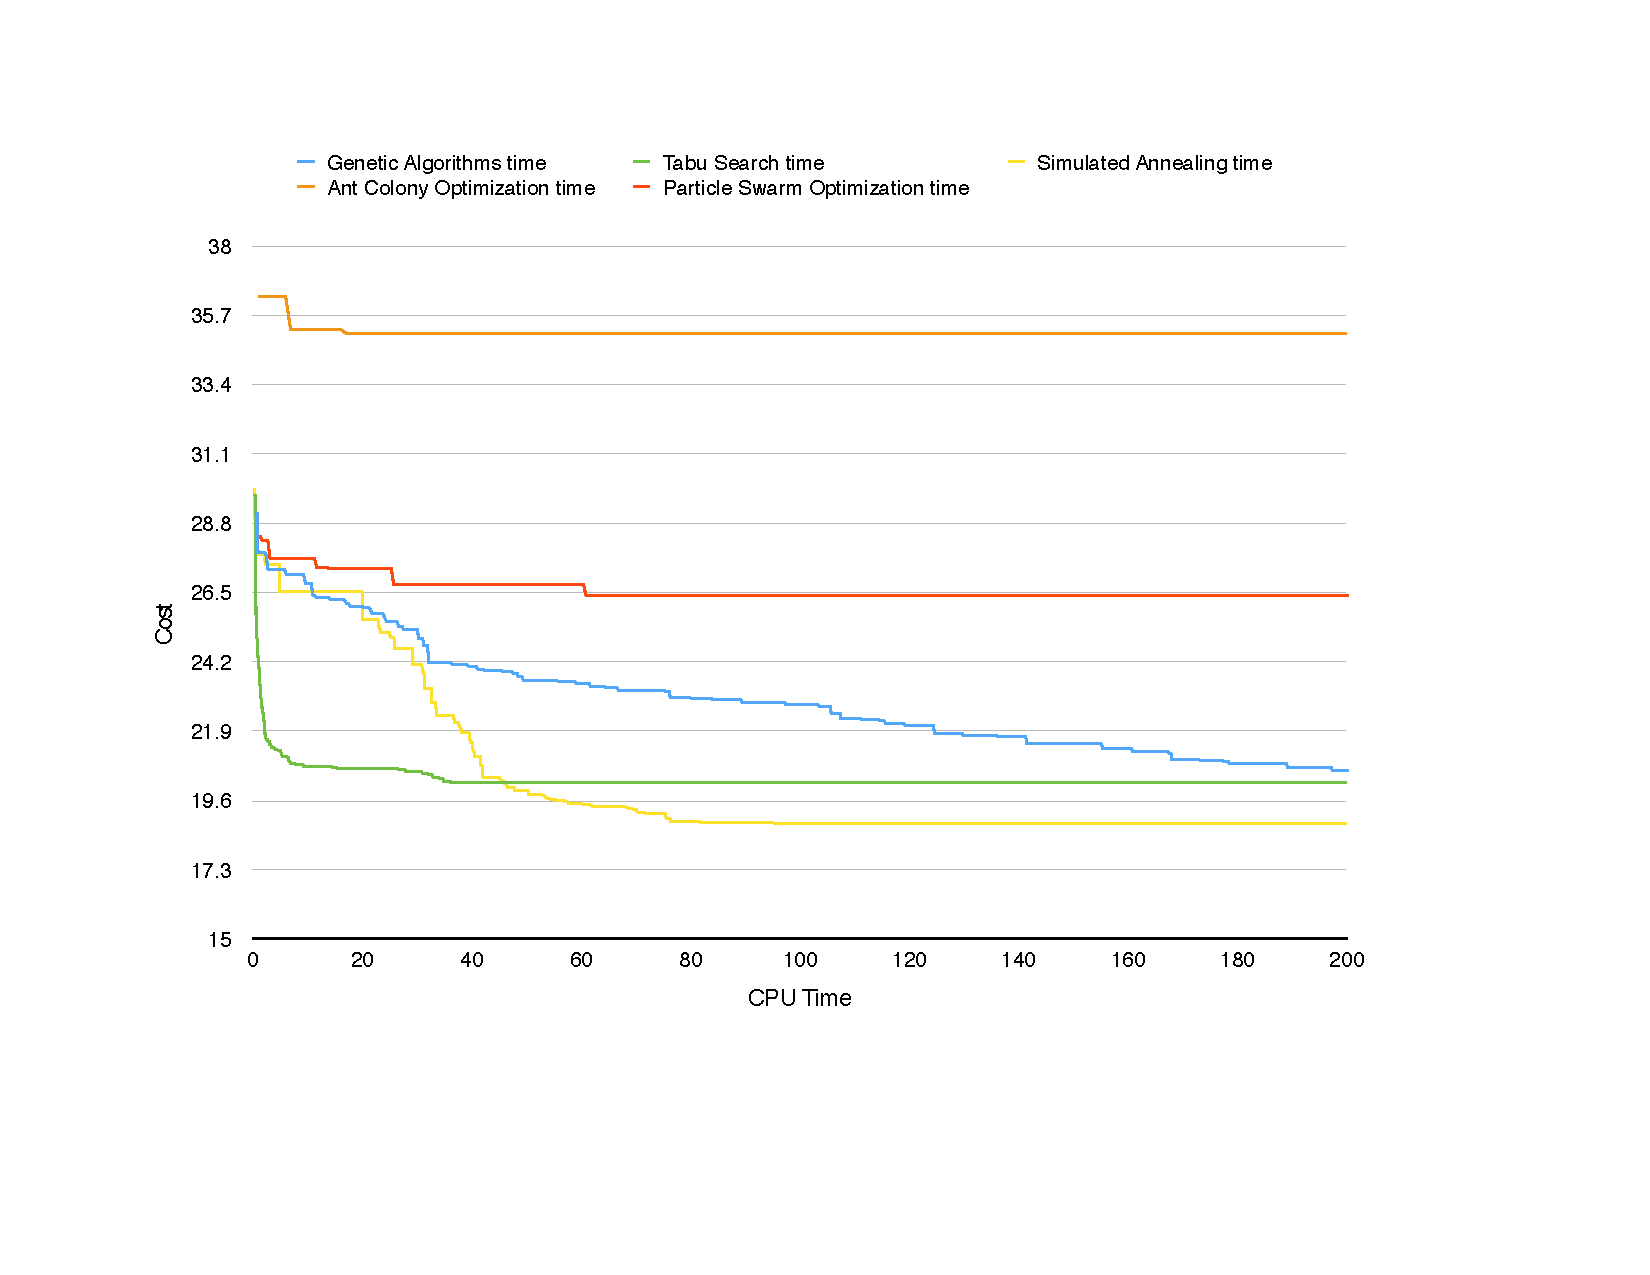
\includegraphics[width=1.2\textwidth]{images/graph.pdf}
}
\caption{Algorithm results for the large dataset}
\end{figure}
\end{center}

\newpage
\section{Conclusions \& Recommendations}

This paper has presented a comparative study of metaheuristic algorithms used within an optimization based approach to solving the MRTA problem. Five metaheuristics were considered: Tabu Search, Simulated Annealing, Genetic Algorithms, Particle Swarm optimization, and Ant Colony Optimization.

We found that our algorithms had varied performance which is quite apparent in Figure 2. Simulated Annealing was our most successful algorithm due to a fast convergence rate with the most optimal solution. Simulated Annealing was known to be effective in solving problems similar to MRTA including Quadratic Assignment in previous papers\cite{Badreldin}, so this is not a particularly surprising discovery.

The more complicated algorithms were the P-Metaheuristic algorithms: Ant Colony Optimization, Particle Swarm Optimization and Genetic Algorithm. None of them had incredible speeds of convergence, though GA did find very strong solutions. These algorithms were the most difficult to implement and optimize so their relatively poor performance is to be expected. Each of these algorithms contains significantly more calculations per iteration and tuning parameters than their simpler alternatives.

This difference in scaling is one of our primary concerns for future study because given algorithms with more effective scaling we may have been able to get better results from the P-Metaheuristic algorithms. Further optimizations are needed to implement these algorithms as efficiently as the S-Metaheuristic algorithms. 

Since we had only intermediate experience writing MATLAB programs, we were unable to optimize our program as thoroughly as expert MATLAB programmers would have been capable. The choice of language also made an tremendously poor impact on speed; faster languages would certainly see hugely improved results. In addition to algorithmic improvements, each method had several internal parameters in need of tuning.

Tuning the algorithms' various parameters was by far the most difficult aspect of the project, owing to the fact that we did not implement adaptive versions of the algorithms. Due to the stochastic nature of these algorithms, a qualitative evaluation of a set of parameters is very hard to perform. The sheer number of parameters also made it difficult to tune effectively because modification of one rarely lead to drastically different results, but modification of many did not lead itself to analysis.

However, as is so often the case, it was modifications of the algorithms themselves that lead to the most drastic changes. For example, the GA algorithm originally used a generational model, but switching to a steady state model lead to much better parents for following generations. Additionally, this change lead to a faster convergence. 

Furthermore, our PSO algorithm was also modified to not persist velocities between iterations. Due to the way velocity was defined, no sense of direction could possibly persist between positions. Thusly, after performing a swap between solutions, velocity would not apply, so it was thrown out entirely. This was one of our breakthroughs in the implementation of this algorithm, and significantly helped lead to convergence.

This comparative study of metaheuristic algorithms revealed some interesting data, and we were able to draw some enlightening conclusions in this report. TS and SA were the most effective algorithms we developed, but the data from small scale problems show that our P-Metaheuristic algorithms are also able to solve MRTA optimization problems.  If better results are required one could create adaptive or cooperative versions of these algorithms in order to tune the algorithms to particular data sets. In conclusion, TS and SA are the most effective algorithms to solve MRTA optimization problems and they are also very easy to implement.

\printbibliography

\end{document}
